\documentclass[12pt]{article}
\usepackage[utf8]{inputenc} % Sin el guion
\usepackage[T1]{fontenc}    % Ayuda a que las tildes se copien bien del PDF
\usepackage[spanish]{babel}
\usepackage{amsmath}
\usepackage{amssymb}
\usepackage{geometry}
\usepackage{csquotes}
\usepackage[backend=biber,style=numeric]{biblatex}
\addbibresource{referenciasExamen.bib}


\geometry{margin=1in}
\usepackage{listings}
\usepackage{xcolor}

\usepackage{graphicx}
\usepackage{float}      % opcional, para usar [H]
\usepackage{hyperref}   % opcional, para referencias clickeables

% \lstset{
%     language=Python,
%     basicstyle=\ttfamily\footnotesize,
%     keywordstyle=\color{blue},
%     commentstyle=\color{gray},
%     stringstyle=\color{black},
%     numbers=left,
%     numberstyle=\tiny,
%     frame=single,
%     rulecolor=\color{black},
%     breaklines=true,
%     showstringspaces=false
% }
\lstset{
    language=Python,
    basicstyle=\ttfamily\scriptsize, % Bajamos un poco el tamaño para que quepa mejor
    keywordstyle=\color{blue},
    commentstyle=\color{gray},
    stringstyle=\color{black},
    numbers=left,
    numberstyle=\tiny,
    frame=single,
    rulecolor=\color{black},
    breaklines=true,           % CORRECCION: Corta las lineas largas automaticamente
    breakatwhitespace=true,    % Solo corta en espacios en blanco para no romper palabras
    showstringspaces=false,
    lineskip=2pt,              % Agrega espacio entre lineas para que no se vea amontonado
    basewidth=0.5em,           % Ancho de los caracteres
    xleftmargin=10pt,          % Margen para que el cuadro no se pegue al texto
    xrightmargin=10pt
}

\hypersetup{
    pdfborder={0 0 0}, % Elimina los rectángulos de colores
    colorlinks=true,   % Activa el color en el texto de la liga
    linkcolor=black,   % Color para referencias internas
    citecolor=black,   % Color para citas bibliográficas
    urlcolor=black     % Color para enlaces web
}


\title{Examen 1. TITANIC }
\author{Ing. Isaias Garcia Zanella}
\date{\today}

\begin{document}

\maketitle

\section{Introducción}
El presente informe detalla el desarrollo e implementación de un modelo de clasificación basado en el algoritmo de K-Vecinos más Cercanos (KNN) para predecir la supervivencia de los pasajeros del Titanic. El análisis se llevó a cabo utilizando dos enfoques de evaluación: la técnica de Hold-out y la validación cruzada de K-pliegues, con el objetivo de comparar su desempeño y obtener una estimación robusta de la capacidad predictiva del modelo y aplicar 
todo lo aprendido en clase duarnte el curso de Machine Learning.

\section{Marco Teórico}
% \subsection{Aprendizaje Maquina (Machine Learning)}
% Tradicionalmente, el diccionario define <<aprender>> de varias maneras, todas ellas relacionadas a procesos humanos de adquision de conocimientos.
% \begin{enumerate}
%     \item Obtener conocimiento ya sea por estudio, experiencia o ensenanza.
%     \item Ser conciente o darse cuenta de cierta informacioon a traves de la observacion.
%     \item Recibir instruccion de manera formal o informal.
%     \item Ser informado acerca de algo.
% \end{enumerate}

% No obstante, cuando trasladamos el concepto al ambito de los sistemas computacionales, surgen ciertas limitaciones y desafios semanticos.

% Sin embargo, una interpretacion pragmatica del aprendizaje de maquina( machine learning), dentro del campo de la inteligencia artificial, puede entenderse como la habilidad de un sistema para mejorar su desempeno en una tarea especifica mediante la experiencia, sin ser explicitamente programado para ello.
% Aqui la << experiencia >> se refiere al uso de datos - conocidos como datos de entrenamiento - que permiten al sistema identificar patrones, regularidades y relaciones, a partir de las cuales se construyen modelos predictivos o descriptivos.
% \cite{De0a100enIA}.

% \subsubsection{Clasificacion del aprendizaje en Inteligencia Artificial}
% En la practica, el aprendizaje maquina se clasifica desde diferentes prespectivas, principalmente:
% \begin{itemize}
%     \item Según la forma en que el modelo aprende los datos: \begin{itemize}
%                 \item Aprendizaje supervisado: El sistema aprende a partir de un conjunto de datos etiquetados, donde cada ejemplo de entrenamiento incluye tanto las características de entrada como la salida deseada. El objetivo es que el modelo generalice a partir de estos ejemplos para predecir la salida correcta para nuevos datos no vistos.
%                 \item Aprendizaje no supervisado: En este caso, el sistema trabaja con datos sin etiquetar, buscando patrones, estructuras o agrupaciones dentro de los datos. El objetivo es descubrir relaciones ocultas o segmentar los datos en grupos similares.
%                 \item Aprendizaje por refuerzo: Aquí, el sistema aprende a través de la interacción con un entorno, recibiendo recompensas o castigos en función de sus acciones. El objetivo es maximizar la recompensa acumulada a lo largo del tiempo.
%             \end{itemize}
%     \item Segun el estilo o enfoque del aprendizaje: \begin{itemize}
%                     \item Aprendizaje inductivo: Generaliza reglas o patrones a partir de ejmplos especificos.
%                     \item APrendizajes deductivos: APlica reglas generales para inferir resultados especificos.
%                     \item Aprendizaje transductivo: No generaliza, sino que predice valores directamente para los casos desconocidos durante el aprendizaje.
%                     \item Aprendizaje en linea vs. por lotes: El aprendizaje puede hacerse de forma continua conforme llegan los datos (en linea) o usando todo el conjunto de datos de una sola vez (por lotes).
%                 \end{itemize}
% \end{itemize}

% \cite{De0a100enIA}


% Al trabajar con algoritmos de aprendizaje automatico, uno de los primeros pasos criticos es la identificacion y comprension de los tipos de datos disponibles. En ciencia de datos, los atributos o variables pueden clasificarse en diversas escalas de medicion:

% \begin{itemize}
%     \item Datos categoricos: Representa categorías sin orden inherente, como el género o la profesión.
%     \item Datos ordinales: Similar a la nominal, pero con un orden específico, como el nivel de educación o la satisfacción del cliente.
%     \item Datos de intervalo: Tiene un orden y distancias significativas entre valores, pero sin un cero absoluto, como la temperatura en Celsius.
%     \item Datos de proporcion: Similar a los de intrevalo, pero con un punto cero absoluto (por ejemplo,peso, edad, ingresos).
% \end{itemize}


% Otro aspecto fundamental en la construccion de modelos de aprendizajes automatico es la diuvison de los datos en diferentes subconjumtos, siendo los principales :
% \begin{itemize}
%     \item Conjunto de entrenamiento : Utilizado para ajustar el modelo; es decir, para que este aprenda los patrones, relaciones y estructuras contenidas en los datos.
%     \item Conjunto de prueba (o validacion) : Empleado para evaluar la capacidad del modelo para generalizar a datos no vistos durante el entrenamiento. Sirve para estimar el rendimiento real del modelo y ajustar hiperparametros.
% \end{itemize}

% \cite{De0a100enIA}

% \subsection{Sobreajuste}
%     El sobreajuste o sobreaprendizaje ocurre cuando un modelo ajusta sus parametros de manera excesiva a los datos de entrnamiento, capturando no solo los patrones verdaderos, sino tambien el ruido, outliers o irregularidades del conjunto. Esto se manifiesta cuando el modelo tiene una precision mu alta en el entrenamiento, pero pobre desempeno en datos de prueba, lo que implica que no generaliza. Las causas mas comunes  para esto son:
%     \begin{itemize}
%         \item Modelos excesivamente complejos.
%         \item Falta de regularizacion.
%         \item Entrenamiento prolongado sin validacion cruzada.
%         \item Conjuntos de datos pequenos o desequilibrados.
%     \end{itemize}

%     Algunas soluciones mas utilizadas para lidiar con el sobreajuste incluyen:
%     \begin{itemize}
%         \item Regularizacion (L1,L2).
%         \item Reduccion de la complejidad del modelo.
%         \item Aumeto del conjunto de datos.
%         \item Validacion cruzada.
%         \item Tecnicas de ensamble.
%     \end{itemize}
% \cite{De0a100enIA}

% \subsection{Subajuste}
%     Por el contrario, el subajuste o subaprendizaje ocurre cuando el modelo no logra aprender correctamente los patrones de los datos, ni siquiera en el conjunto de entrenamiento.
%     Esto significa que el modelo es demasiado simple o mal configurado para capturar la complejidad del problema. algunas de las causas mas comunes son las siguientes: 
%     \begin{itemize}
%         \item Modelos muy simples( como una regresion lineal para datos no lineales)
%         \item Insuficiente entrenamiento (muy pocas epocas o iteraciones).
%         \item Hiperparametros mal seleccionados.
%         \item Transformacion inadecuada de los datos.
%     \end{itemize}

%     Algunas soluciones mas utilizadas para lidiar con el subajuste incluyen:
%     \begin{itemize}
%         \item Aumentar la complejidad del modelo.
%         \item Mejorar la ingenieria de caracteristicas.
%         \item Aumentar el tiempo de entrenamiento.
%         \item Revisar los supuestos del modelo frente a la naturaleza de los datos.
%     \end{itemize}
% \cite{De0a100enIA}
\subsection{Aprendizaje Máquina (Machine Learning)}
Tradicionalmente, el diccionario define <<aprender>> de varias maneras, todas ellas relacionadas a procesos humanos de adquisición de conocimientos.
\begin{enumerate}
    \item Obtener conocimiento ya sea por estudio, experiencia o enseñanza.
    \item Ser consciente o darse cuenta de cierta información a través de la observación.
    \item Recibir instrucción de manera formal o informal.
    \item Ser informado acerca de algo.
\end{enumerate}

No obstante, cuando trasladamos el concepto al ámbito de los sistemas computacionales, surgen ciertas limitaciones y desafíos semánticos.

Sin embargo, una interpretación pragmática del aprendizaje de máquina (machine learning), dentro del campo de la inteligencia artificial, puede entenderse como la habilidad de un sistema para mejorar su desempeño en una tarea específica mediante la experiencia, sin ser explícitamente programado para ello.
Aquí la << experiencia >> se refiere al uso de datos —conocidos como datos de entrenamiento— que permiten al sistema identificar patrones, regularidades y relaciones, a partir de las cuales se construyen modelos predictivos o descriptivos.
\cite{De0a100enIA}.

Este proceso de aprendizaje se fundamenta en la optimización de una función objetivo, donde el algoritmo ajusta sus parámetros internos para minimizar el error entre sus predicciones y la realidad observada. En este contexto, el algoritmo no solo almacena información, sino que desarrolla la capacidad de inducción, permitiéndole tomar decisiones sobre datos que nunca ha procesado anteriormente \cite{bishop2006pattern}.

\subsubsection{Clasificación del aprendizaje en Inteligencia Artificial}
En la práctica, el aprendizaje máquina se clasifica desde diferentes perspectivas, principalmente:
\begin{itemize}
    \item Según la forma en que el modelo aprende los datos: \begin{itemize}
                \item Aprendizaje supervisado: El sistema aprende a partir de un conjunto de datos etiquetados, donde cada ejemplo de entrenamiento incluye tanto las características de entrada como la salida deseada. El objetivo es que el modelo generalice a partir de estos ejemplos para predecir la salida correcta para nuevos datos no vistos.
                \item Aprendizaje no supervisado: En este caso, el sistema trabaja con datos sin etiquetar, buscando patrones, estructuras o agrupaciones dentro de los datos. El objetivo es descubrir relaciones ocultas o segmentar los datos en grupos similares.
                \item Aprendizaje por refuerzo: Aquí, el sistema aprende a través de la interacción con un entorno, recibiendo recompensas o castigos en función de sus acciones. El objetivo es maximizar la recompensa acumulada a lo largo del tiempo.
            \end{itemize}
    \item Según el estilo o enfoque del aprendizaje: \begin{itemize}
                    \item Aprendizaje inductivo: Generaliza reglas o patrones a partir de ejemplos específicos.
                    \item Aprendizajes deductivos: Aplica reglas generales para inferir resultados específicos.
                    \item Aprendizaje transductivo: No generaliza, sino que predice valores directamente para los casos desconocidos durante el aprendizaje.
                    \item Aprendizaje en línea vs. por lotes: El aprendizaje puede hacerse de forma continua conforme llegan los datos (en línea) o usando todo el conjunto de datos de una sola vez (por lotes).
                \end{itemize}
\end{itemize}

\cite{De0a100enIA}

Cabe destacar que la elección entre estos enfoques depende directamente de la naturaleza del problema y la disponibilidad de etiquetas. Por ejemplo, en problemas de clasificación binaria como la predicción de supervivencia, el aprendizaje supervisado es el estándar, mientras que el análisis de perfiles de clientes suele abordarse mediante el aprendizaje no supervisado \cite{hastie2009elements}.


Al trabajar con algoritmos de aprendizaje automático, uno de los primeros pasos críticos es la identificación y comprensión de los tipos de datos disponibles. En ciencia de datos, los atributos o variables pueden clasificarse en diversas escalas de medición:

\begin{itemize}
    \item Datos categóricos: Representan categorías sin orden inherente, como el género o la profesión.
    \item Datos ordinales: Similares a los nominales, pero con un orden específico, como el nivel de educación o la satisfacción del cliente.
    \item Datos de intervalo: Tienen un orden y distancias significativas entre valores, pero sin un cero absoluto, como la temperatura en Celsius.
    \item Datos de proporción: Similares a los de intervalo, pero con un punto cero absoluto (por ejemplo, peso, edad, ingresos).
\end{itemize}

La correcta identificación de estas escalas permite determinar el preprocesamiento adecuado, como la aplicación de técnicas de codificación (\textit{one-hot encoding}) para datos categóricos o la normalización para datos de proporción, asegurando que el modelo no asuma erróneamente un orden o importancia superior debido a la magnitud de las escalas numéricas \cite{james2013introduction}.


Otro aspecto fundamental en la construcción de modelos de aprendizaje automático es la división de los datos en diferentes subconjuntos, siendo los principales:
\begin{itemize}
    \item Conjunto de entrenamiento: Utilizado para ajustar el modelo; es decir, para que este aprenda los patrones, relaciones y estructuras contenidas en los datos.
    \item Conjunto de prueba (o validación): Empleado para evaluar la capacidad del modelo para generalizar a datos no vistos durante el entrenamiento. Sirve para estimar el rendimiento real del modelo y ajustar hiperparámetros.
\end{itemize}

\cite{De0a100enIA}

Para garantizar una evaluación robusta y mitigar el sesgo introducido por una única partición aleatoria, se recomienda el uso de técnicas como la validación cruzada de K-pliegues (\textit{K-Fold Cross Validation}). Este método permite que cada dato del conjunto participe tanto en el entrenamiento como en la validación, proporcionando una estimación más precisa del desempeño del modelo en el mundo real \cite{raschka2015python}.

\subsection{Sobreajuste}
    El sobreajuste o sobreaprendizaje ocurre cuando un modelo ajusta sus parámetros de manera excesiva a los datos de entrenamiento, capturando no solo los patrones verdaderos, sino también el ruido, outliers o irregularidades del conjunto. Esto se manifiesta cuando el modelo tiene una precisión muy alta en el entrenamiento, pero pobre desempeño en datos de prueba, lo que implica que no generaliza. Las causas más comunes para esto son:
    \begin{itemize}
        \item Modelos excesivamente complejos.
        \item Falta de regularización.
        \item Entrenamiento prolongado sin validación cruzada.
        \item Conjuntos de datos pequeños o desequilibrados.
    \end{itemize}

    Algunas soluciones más utilizadas para lidiar con el sobreajuste incluyen:
    \begin{itemize}
        \item Regularización (L1, L2).
        \item Reducción de la complejidad del modelo.
        \item Aumento del conjunto de datos.
        \item Validación cruzada.
        \item Técnicas de ensamble.
    \end{itemize}
\cite{De0a100enIA}

\subsection{Subajuste}
    Por el contrario, el subajuste o subaprendizaje ocurre cuando el modelo no logra aprender correctamente los patrones de los datos, ni siquiera en el conjunto de entrenamiento.
    Esto significa que el modelo es demasiado simple o está mal configurado para capturar la complejidad del problema. Algunas de las causas más comunes son las siguientes: 
    \begin{itemize}
        \item Modelos muy simples (como una regresión lineal para datos no lineales).
        \item Insuficiente entrenamiento (muy pocas épocas o iteraciones).
        \item Hiperparámetros mal seleccionados.
        \item Transformación inadecuada de los datos.
    \end{itemize}

    Algunas soluciones más utilizadas para lidiar con el subajuste incluyen:
    \begin{itemize}
        \item Aumentar la complejidad del modelo.
        \item Mejorar la ingeniería de características.
        \item Aumentar el tiempo de entrenamiento.
        \item Revisar los supuestos del modelo frente a la naturaleza de los datos.
    \end{itemize}
\cite{De0a100enIA}

% \subsection{Aprendizaje Basado en Similitud}
%     El aprendizaje basado en similitud en machine learning fundamenta su paradigma en el principio heuristico de que patrones historicos existosos constituyen
% predicadores confiables para instancias futuras. Es decir, el aprendizaje basado en similitud en lo que refiere a aprendizaje maquina tiene su origen en la idea de que la mejor manera de realizar una prediccion o clasificacion es simplemente observar lo que ha funcionado
% bien anteriormente y predecir el mismo comportamiento de nuevo.

%     El modelo de aprendizaje maquina basados en similitud mas popular es el algoritmo por K-Vecions mas cercanos - << KNN>> o <<N- Nearest Neighbors>> -. Este tambien puede considerarse un modelo de clasificacion.
%     El algoritmo KNN implementa un enfoque de aprendizaje perezoso, - lazy learning - donde la fase de entrenamiento se reduce a almacenar el conjunto completo de instancias etiquetdadas D = \begin{math}
%     \{(x_1,y_1), (x_2,y_2), ..., (x_n,y_n)\}
%     \end{math}. Durante la inferencia, para nueva instancia, el algoritmo ejecuta:
%     \cite{hastie2009elements}.  
%     \begin{enumerate}
%         \item Calculo de distancia: Computa \begin{math}
%             d(x_query,x_i)
%             \end{math} para todos los puntos de entrenamiento.
%         \item Selección de los K vecinos más cercanos.
%         \item Clasificación o predicción basada en la votación mayoritaria (para clasificación) o el promedio (para regresión).
%     \end{enumerate}
%     \cite{De0a100enIA}

\subsection{Aprendizaje Basado en Similitud}
El aprendizaje basado en similitud en \textit{machine learning} fundamenta su paradigma en el principio heurístico de que los patrones históricos exitosos constituyen predictores confiables para instancias futuras. Es decir, este enfoque parte de la premisa de que la mejor manera de realizar una predicción o clasificación es identificar instancias pasadas con características similares a la consulta actual y proyectar un comportamiento análogo.

A diferencia de los modelos basados en parámetros que intentan resumir los datos en una función matemática, los modelos de similitud mantienen una relación directa con las instancias individuales del conjunto de datos. El modelo de aprendizaje máquina basado en similitud más popular es el algoritmo de K-Vecinos más cercanos (\textit{K-Nearest Neighbors} o KNN). Este algoritmo es ampliamente reconocido por su simplicidad y eficacia en tareas de clasificación y regresión \cite{bishop2006pattern}.

El algoritmo KNN implementa un enfoque de aprendizaje perezoso (\textit{lazy learning}), donde la fase de entrenamiento se reduce esencialmente a almacenar el conjunto completo de instancias etiquetadas $D = \{(x_1, y_1), (x_2, y_2), \dots, (x_n, y_n)\}$. Al no generar un modelo discriminativo explícito durante el entrenamiento, el costo computacional se traslada a la fase de inferencia. Durante esta etapa, para una nueva instancia de consulta ($x_{query}$), el algoritmo ejecuta los siguientes pasos:
\cite{hastie2009elements}.



\begin{enumerate}
    \item \textbf{Cálculo de distancia:} Computa la métrica de proximidad $d(x_{query}, x_i)$ para todos los puntos del conjunto de entrenamiento. Las métricas más comunes incluyen la distancia Euclidiana, la distancia de Manhattan y la distancia de Minkowski.
    \item \textbf{Selección de vecinos:} Identifica los $K$ puntos más cercanos a $x_{query}$ basándose en las distancias calculadas.
    \item \textbf{Votación o promedio:} Realiza la clasificación mediante una votación mayoritaria entre las etiquetas de los $K$ vecinos, o una predicción de valor continuo mediante el promedio de los mismos en casos de regresión.
\end{enumerate}

La efectividad del algoritmo KNN depende críticamente de dos factores: la elección del valor $K$ y la métrica de distancia empleada. Un valor de $K$ demasiado pequeño puede hacer que el modelo sea sensible al ruido (sobreajuste), mientras que un valor demasiado grande puede suavizar excesivamente las fronteras de decisión, ignorando patrones locales importantes (subajuste). Asimismo, dado que KNN se basa en distancias, es fundamental realizar una normalización o estandarización previa de las características para evitar que aquellas con magnitudes mayores dominen el cálculo de la similitud \cite{raschka2015python}.

\cite{De0a100enIA}

\subsection{Métricas de evaluación}

La evaluación del desempeño de un modelo de clasificación es un paso crítico para determinar su capacidad de generalización. La base fundamental para el cálculo de la mayoría de estas métricas es la \textit{Matriz de Confusión}, una tabla que desglosa las predicciones del modelo en cuatro categorías: Verdaderos Positivos (VP), Verdaderos Negativos (VN), Falsos Positivos (FP) y Falsos Negativos (FN) \cite{fawcett2006introduction}.



A partir de esta matriz, se derivan las siguientes métricas de evaluación:

\begin{itemize}
    \item \textbf{Exactitud (Accuracy):} Es la proporción de predicciones correctas (tanto positivas como negativas) respecto al total de casos. Aunque es la métrica más intuitiva, puede ser engañosa en conjuntos de datos desequilibrados.
    \[ \text{Accuracy} = \frac{VP + VN}{VP + VN + FP + FN} \]

    \item \textbf{Precisión (Precision):} Indica la calidad de las predicciones positivas. Es la fracción de casos identificados como positivos que realmente lo son. Es crucial cuando el costo de un Falso Positivo es alto.
    \[ \text{Precision} = \frac{VP}{VP + FP} \]

    \item \textbf{Sensibilidad (Recall / Exhaustividad):} Mide la capacidad del modelo para detectar todos los casos positivos reales. En el contexto del Titanic, un \textit{recall} alto significaría que el modelo no "olvida" a los sobrevivientes reales.
    \[ \text{Recall} = \frac{VP}{VP + FN} \]

    \item \textbf{Especificidad:} Representa la tasa de verdaderos negativos; es decir, la capacidad del modelo para identificar correctamente los casos de la clase negativa (quienes no sobrevivieron).
    \[ \text{Especificidad} = \frac{VN}{VN + FP} \]

    \item \textbf{Puntaje F-Beta ($F_\beta$):} Es una generalización del F1-Score que permite ponderar la importancia de la precisión frente al \textit{recall} mediante un parámetro $\beta$. Si $\beta = 1$, obtenemos el F1-Score (media armónica balanceada). Si $\beta > 1$, se le da más importancia a la sensibilidad.
    \[ F_\beta = (1 + \beta^2) \cdot \frac{\text{Precision} \cdot \text{Recall}}{(\beta^2 \cdot \text{Precision}) + \text{Recall}} \]

    \item \textbf{Área bajo la Curva ROC (AUC-ROC):} La curva ROC (\textit{Receiver Operating Characteristic}) representa la tasa de verdaderos positivos frente a la tasa de falsos positivos. El AUC proporciona un valor agregado que mide la capacidad del modelo para distinguir entre clases independientemente del umbral de decisión \cite{hastie2009elements}.
\end{itemize}

La elección de la métrica adecuada depende del objetivo del análisis. En presencia de conjuntos de datos con clases minoritarias, métricas como el F-Score o el AUC suelen ser preferibles sobre la exactitud simple, ya que proporcionan una visión más holística del equilibrio entre errores de Tipo I y Tipo II \cite{japkowicz2011evaluating}.

\subsection{Validación Cruzada de K-Pliegues (K-Fold Cross Validation)}
La validación cruzada de K-pliegues es una técnica robusta de evaluación de modelos que busca mitigar el sesgo introducido por una partición única de los datos. En lugar de depender de una sola división de entrenamiento y prueba, el conjunto de datos se divide en $K$ subconjuntos o "pliegues" de tamaño aproximadamente igual \cite{james2013introduction}.

El proceso se ejecuta de manera iterativa $K$ veces, siguiendo esta lógica:
\begin{enumerate}
    \item En cada iteración $i$, el pliego $k_i$ se reserva para la validación del modelo.
    \item Los restantes $K-1$ pliegues se utilizan para la fase de entrenamiento.
    \item Se calcula la métrica de desempeño (como el \textit{accuracy} o el error) para dicha iteración.
\end{enumerate}



Al finalizar las iteraciones, el rendimiento del modelo se estima mediante el promedio de las métricas obtenidas en cada pliegue. Este enfoque garantiza que cada instancia del dataset participe tanto en el entrenamiento como en la prueba, proporcionando una estimación de la precisión mucho más estable y confiable, especialmente en conjuntos de datos de tamaño limitado como el del Titanic \cite{raschka2015python}.

\subsection{Método del Codo (Elbow Method) para la Optimización de K}
En el algoritmo KNN, la elección del hiperparámetro $K$ (número de vecinos) es determinante para el equilibrio entre el sesgo y la varianza. El método del codo es una técnica heurística utilizada para identificar el valor óptimo de $K$ mediante el análisis de la tasa de error o la precisión en función de diferentes valores de vecindad.

El procedimiento consiste en graficar el desempeño del modelo frente a un rango de valores de $K$ (por ejemplo, de 1 a 31). A medida que $K$ aumenta, la curva de error tiende a descender inicialmente; sin embargo, existe un punto donde la mejora en el rendimiento se vuelve marginal o comienza a degradarse debido al sobreajuste o subajuste.

Este punto de inflexión en la curva, donde el cambio de pendiente es más pronunciado, se denomina "codo". Seleccionar el valor de $K$ en esta región permite obtener un modelo que generaliza correctamente, evitando la complejidad innecesaria de un $K$ muy grande y la sensibilidad al ruido de un $K$ extremadamente pequeño \cite{shalev2014understanding}.

\section{Materiales y Métodos}

La base de datos con la que vamos a trabajar es el conjunto de datos del Titanic, disponible en la plataforma Kaggle. Este dataset contiene información detallada sobre los pasajeros del Titanic, incluyendo características como edad, género, clase de boleto, tarifa pagada, entre otras, así como la variable objetivo que indica si el pasajero sobrevivió o no al desastre.
El análisis se llevará a cabo utilizando Python, con bibliotecas especializadas en ciencia de datos como \textit{pandas} para la manipulación de datos y la evaluación del modelo, y \textit{matplotlib} para la visualización de resultados. El proceso metodológico incluirá las siguientes etapas:
\begin{itemize}
    \item \textbf{Preprocesamiento de datos:} Limpieza de datos, manejo de valores faltantes, codificación de variables categóricas y normalización de características numéricas.
    \item \textbf{División del dataset:} Separación del conjunto de datos en entrenamiento y prueba, utilizando una proporción estándar (por ejemplo, 80\% para entrenamiento y 20\% para prueba).
    \item \textbf{Entrenamiento del modelo:} Implementación del algoritmo KNN utilizando clases, con una búsqueda de hiperparámetros para determinar el valor óptimo de $K$ mediante el método del codo.
    \item \textbf{Evaluación del modelo:} Cálculo de métricas.
    \item \textbf{Validación cruzada:} Aplicación de la validación cruzada de K-pliegues para obtener una estimación más robusta del desempeño del modelo.
    \item \textbf{Visualización de resultados:} Creación de gráficos para ilustrar la relación entre el valor de $K$ y las métricas de desempeño, así como la matriz de confusión para evaluar la distribución de predicciones.
\end{itemize}

Ahora pasaremos a explicar algunas funciones que se utilizarán en el código para la implementación del modelo KNN y la evaluación de su desempeño. Cabe mencionar que se utilizaron algunas funciones previamnete creadas para la codificacion y normalizacion de datos en algunas columnas, esto para que el modelo pueda tener una mayor eficacia al realizar el entrenamiento, comentado esto ahora si continuaremos con la implementacion del algoritmo KNN.


\subsection{Implementación del Algoritmo KNN}

Para el desarrollo de este proyecto, se optó por una implementación propia del clasificador de K-Vecinos más Cercanos dentro del entorno de Python. La arquitectura de la clase \texttt{KNeighbors\_Classifier} sigue el paradigma de programación orientada a objetos (POO) y se estructura bajo los tres pilares fundamentales del algoritmo: almacenamiento de datos (\textit{Lazy Learning}), cálculo de distancias y votación mayoritaria.

\subsubsection{Descripción de la Clase y Métodos}

\begin{itemize}
    \item \textbf{Constructor (\texttt{\_\_init\_\_}):} Define el hiperparámetro $k$, que representa el número de vecinos a considerar para la clasificación.
    \item \textbf{Método \texttt{fit}:} A diferencia de otros modelos, el entrenamiento en KNN es pasivo. En este método se realiza la asignación del conjunto de entrenamiento a la memoria del objeto, almacenando las dimensiones de la matriz de características.
    \item \textbf{Método \texttt{euclidean}:} Implementa la métrica de distancia euclidiana entre dos vectores utilizando la norma $L^2$. Esta función es el núcleo geométrico del algoritmo.
    \item \textbf{Método \texttt{find\_neighbors}:} Ejecuta el cálculo de distancias desde un punto de consulta hacia todas las instancias de entrenamiento. Posteriormente, utiliza \texttt{argsort} para obtener los índices de las $k$ distancias más pequeñas y retorna sus etiquetas correspondientes.
    \item \textbf{Método \texttt{predict}:} Orquesta la inferencia para múltiples instancias de prueba. Para cada dato, identifica sus vecinos y aplica la función estadística \texttt{mode} (moda) para determinar la clase ganadora por mayoría de votos.
\end{itemize}

\subsubsection{Código Fuente del Clasificador}

\begin{minipage}{0.9\textwidth}
\begin{lstlisting}[caption={Implementación manual del clasificador KNN en Python}]
class KNeighbors_Classifier():
    def __init__(self, k):
        self.k = k
        
    def fit(self, X_train, Y_train):
        self.X_train = X_train
        self.Y_train = Y_train
        self.m, self.n = X_train.shape
        
    def predict(self, X_test):
        m_test = X_test.shape[0]
        Y_predict = np.zeros(m_test)
        for i in range(m_test):
            neighbors_labels = self.find_neighbors(X_test[i])
            # Se calcula la moda para la votacion mayoritaria
            m = mode(neighbors_labels, keepdims=True)
            Y_predict[i] = m.mode.flatten()[0]
        
        return Y_predict

    def find_neighbors(self, x):
        euclidean_distances = np.zeros(self.m)
        for i in range(self.m):
            d = self.euclidean(x, self.X_train[i])
            euclidean_distances[i] = d
        
        # Obtener indices que ordenan las distancias de menor a mayor
        inds = euclidean_distances.argsort()
        # Ordenamos las etiquetas segun la cercania
        Y_train_sorted = self.Y_train[inds]
        return Y_train_sorted[:self.k]

    def euclidean(self, x, x_train):
        # Implementacion matematica de la distancia euclidiana
        return np.sqrt(np.sum(np.square(x - x_train)))
\end{lstlisting}
\end{minipage}

\subsection{Estrategias de Partición y Validación de Datos}

Para evaluar la capacidad de generalización del clasificador KNN, se implementaron dos estrategias distintas de partición de datos. El objetivo de este enfoque dual es contrastar una evaluación estática frente a una validación dinámica y exhaustiva.

\subsubsection{División Estática de Datos (Hold-out Validation)}

La primera aproximación para la evaluación del modelo consiste en el método de \textit{Hold-out}, el cual separa el conjunto de datos en dos bloques independientes. Esta técnica permite entrenar el algoritmo en una porción mayoritaria de la muestra y reservar un porcentaje menor para validar su desempeño final, garantizando que el modelo no sea evaluado con los mismos datos que conoció durante el entrenamiento.

Para asegurar que los resultados sean reproducibles, se implementa una semilla aleatoria (\textit{random seed}). Esto es fundamental en el ámbito académico, ya que permite que otros investigadores obtengan la misma partición exacta de datos.

\begin{minipage}{0.9\textwidth}
\begin{lstlisting}[caption={Función para la separación estática de datos}]
def separar_datos(df, objetivo, test_size=0.2, random_state=42):
    # Definir una semilla para que los resultados sean reproducibles
    np.random.seed(random_state)
    
    # Mezclar los indices del DataFrame
    indices = df.index.tolist()
    np.random.shuffle(indices)
    
    # Calcular cuantos datos van para test
    tamano_test = int(len(df) * test_size)
    
    # Dividir los indices
    indices_test = indices[:tamano_test]
    indices_train = indices[tamano_test:]
    
    # Crear los sets de entrenamiento y prueba
    train_df = df.loc[indices_train]
    test_df = df.loc[indices_test]
    
    # Separar en X (caracteristicas) y Y (lo que queremos predecir)
    X_train = train_df.drop(columns=[objetivo]).values
    Y_train = train_df[objetivo].values
    X_test = test_df.drop(columns=[objetivo]).values
    Y_test = test_df[objetivo].values
    
    return X_train, X_test, Y_train, Y_test, indices_test
\end{lstlisting}
\end{minipage}

\subsubsection{Validación Cruzada (K-Fold Cross Validation)}

Como método de validación avanzada, se implementó la técnica de \textit{K-Fold Cross Validation}. A diferencia de la partición estática, este procedimiento divide el dataset en $K$ subconjuntos o pliegues. El proceso se repite $K$ veces, rotando en cada iteración el pliegue que funciona como conjunto de prueba.

La función \texttt{validacion\_k\_fold\_retornar\_modelo} ha sido diseñada no solo para calcular la estabilidad del algoritmo, sino para identificar y extraer la instancia del modelo que presenta el mejor desempeño (\textit{accuracy}) histórico. Esto permite mitigar el riesgo de sesgo por selección y proporciona una visión integral de la capacidad predictiva del sistema sobre toda la población de datos disponible.

\begin{minipage}{0.9\textwidth}
\begin{lstlisting}[caption={Función para validación cruzada y selección del mejor modelo},label={lst:validacion_kfold}]
def validacion_k_fold_retornar_modelo(df, objetivo, k_folds=5, k_vecinos=5):
    indices = df.index.tolist()
    np.random.seed(42)
    np.random.shuffle(indices)
    
    folds_indices = np.array_split(indices, k_folds)
    
    mejor_accuracy = 0
    mejor_modelo = None
    mejores_indices_test = None
    lista_accuracy = []

    for i in range(k_folds):
        indices_test = folds_indices[i]
        indices_train = np.concatenate([folds_indices[j] for j in range(k_folds) if j != i])
        
        # Separacion de datos
        train_df = df.loc[indices_train]
        test_df = df.loc[indices_test]
        
        X_train = train_df.drop(columns=[objetivo]).values
        Y_train = train_df[objetivo].values
        X_test = test_df.drop(columns=[objetivo]).values
        Y_test = test_df[objetivo].values
        
        # Entrenar modelo
        modelo_actual = KNeighbors_Classifier(k=k_vecinos)
        modelo_actual.fit(X_train, Y_train)
        
        # Validar
        predicciones = modelo_actual.predict(X_test)
        accuracy_actual = np.mean(predicciones == Y_test)
        lista_accuracy.append(accuracy_actual)
        
        # GUARDAR EL MEJOR
        if accuracy_actual > mejor_accuracy:
            mejor_accuracy = accuracy_actual
            mejor_modelo = modelo_actual
            mejores_indices_test = indices_test
            
    return mejor_modelo, mejores_indices_test, lista_accuracy
\end{lstlisting}
\end{minipage}

\subsection{Optimización del Hiperparámetro K (Curva de Desempeño)}

La selección del valor óptimo de $K$ es un proceso empírico que busca maximizar la capacidad predictiva del modelo. Un valor de $K$ muy bajo puede conducir a un sobreajuste (\textit{overfitting}) debido a la sensibilidad al ruido, mientras que un $K$ excesivamente elevado puede generar un subajuste (\textit{underfitting}) al ignorar estructuras locales en los datos.

Para determinar el valor ideal, se implementó un proceso de iteración sistemática sobre un rango de valores de $K \in [1, 20]$. En cada iteración, se entrena el modelo y se evalúa su desempeño frente al conjunto de prueba, registrando la tasa de acierto (\textit{accuracy rate}). Los resultados se visualizan mediante una gráfica de línea que permite identificar el "punto de codo" o la zona de mayor estabilidad.

\begin{minipage}{0.9\textwidth}
\begin{lstlisting}[caption={Algoritmo de búsqueda del valor K óptimo y visualización de resultados}]
range_used = range(1, 21)
acierto_rate = []

for i in range_used:
    # Se instancia el modelo con el valor actual de K
    knn = KNeighbors_Classifier(k=i)
    knn.fit(X_train, Y_train)
    pred_i = knn.predict(X_test)
    
    # Se calcula la tasa de acierto y se almacena
    acierto_rate.append(np.mean(pred_i == Y_test))

# Graficamos los resultados para analisis visual
plt.figure(figsize=(10,6))
plt.plot(range_used, acierto_rate, 
    color='blue', 
    linestyle='dashed', 
    marker='o', markerfacecolor='red', markersize=10)

# Ajuste de etiquetas en el eje X para mayor precision
plt.xticks(range_used) 
plt.title('Tasa de Acierto vs. Valor de K')
plt.xlabel('K')
plt.ylabel('Tasa de Acierto')
plt.show()
\end{lstlisting}
\end{minipage}


\section{Resultados y Discusión}

Antes de empezar a entrenar el modelo debemos de observar primero como se ve de forma visual las personas que sobrevivieron y las que no, esto para tener una idea de como se ve el dataset y asi poder identificar patrones visuales que puedan ayudar al modelo a realizar una mejor prediccion.

\begin{figure}[H]
    \centering
    \begin{minipage}{0.48\textwidth}
        \centering
        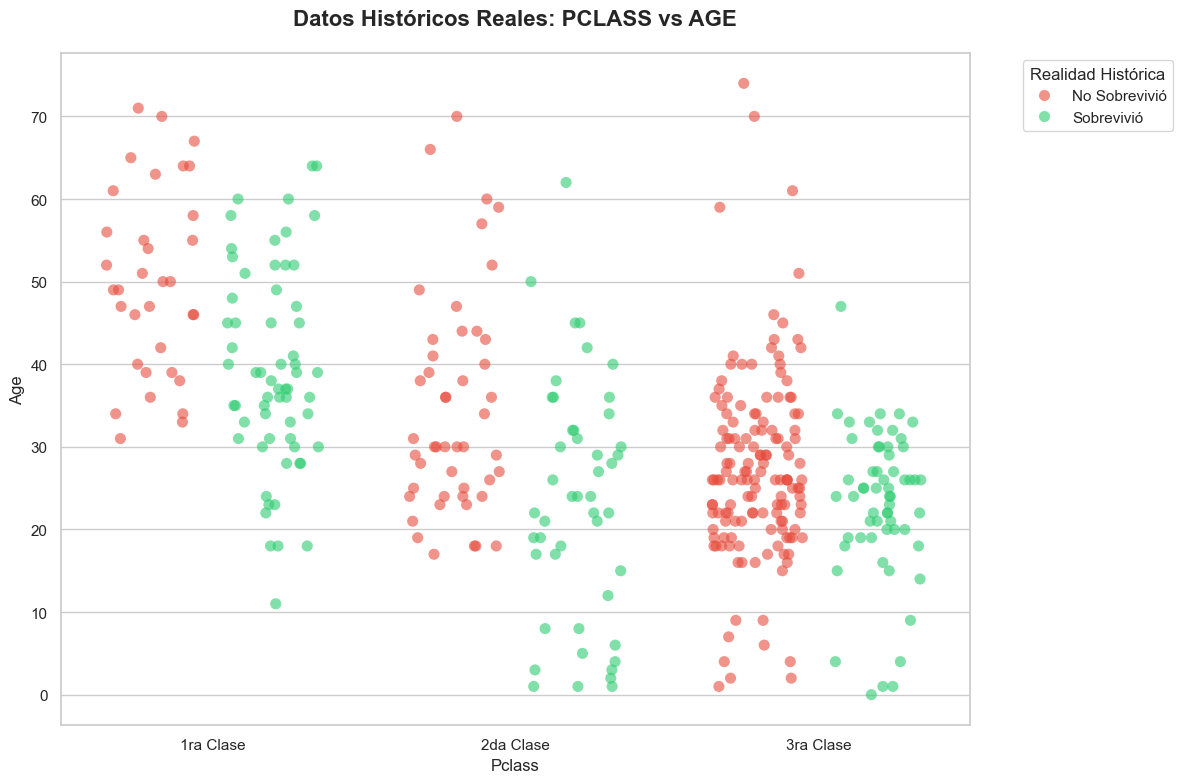
\includegraphics[width=\linewidth]{../Imagenes/Examen1/DistribucionOriginal_ClaseVsEdad.png}
        \caption{ Distribución de sobrevivientes vs no sobrevivientes en función de la edad y clase Social.}
        \label{fig:Distr_Original_ClaseVsEdad}
    \end{minipage}\hfill
    \begin{minipage}{0.48\textwidth}
        \centering
        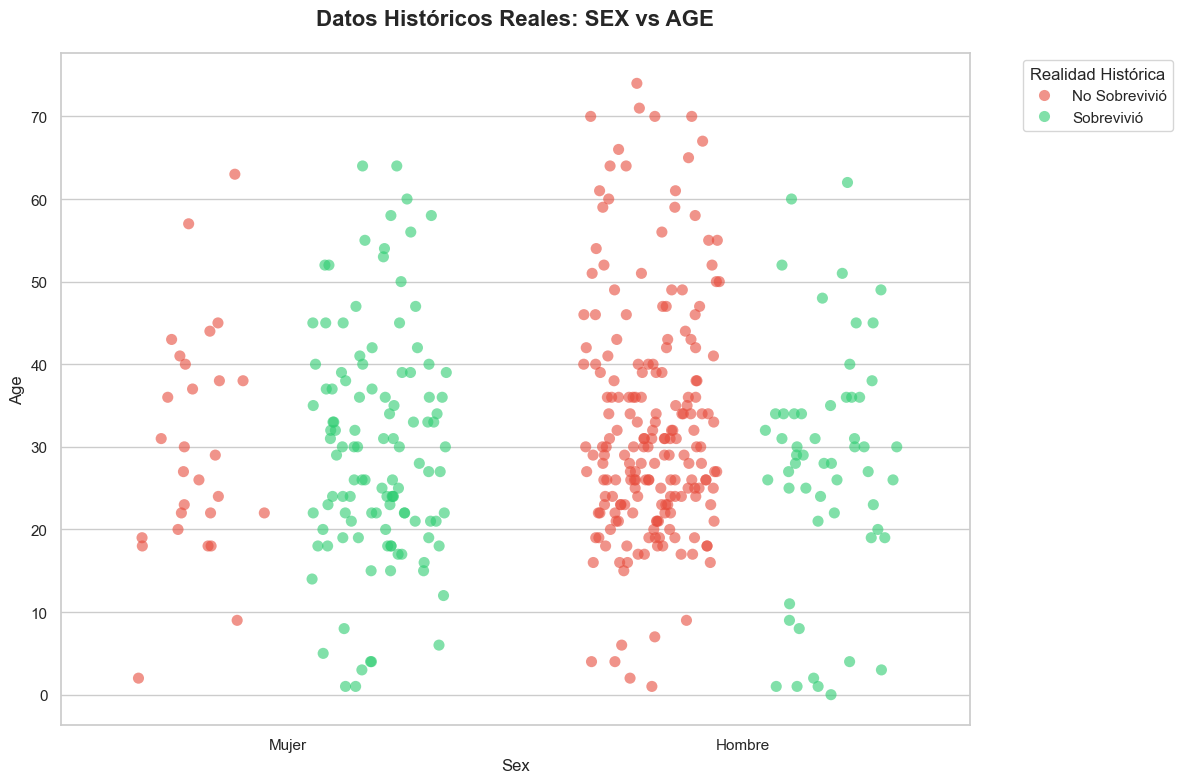
\includegraphics[width=\linewidth]{../Imagenes/Examen1/DistrribucionOrig_GeneroVsEdad.png}
        \caption{ Distribución de sobrevivientes vs no sobrevivientes en función de la edad y Genero.}
        \label{fig:Distr_Original_GeneroVsEdad}
    \end{minipage}
\end{figure}

Con esto podemos observar que la mayoria de los sobrevivientes eran mujeres y niños, esto se puede observar en la grafica de la izquierda, donde se muestra que las personas de clase social mas alta tenian una mayor tasa de supervivencia, y en la grafica de la derecha se observa que las mujeres tenian una mayor tasa de supervivencia que los hombres, esto es un patron visual que el modelo puede identificar para realizar una mejor prediccion.


Una vez observado esto, ahora se procederá a presentar algunos de los métodos utilizados para la implementación del modelo KNN y la evaluación de su desempeño, se procederá a presentar los resultados obtenidos a partir de la aplicación de estas técnicas sobre el dataset del Titanic. Se analizarán las métricas de desempeño, la curva de acierto en función del valor de $K$, y se discutirá la interpretación de estos resultados en el contexto del problema planteado.

\subsection{ Primera prueba.- KNN y Hold-out Validation}
Despues de discriminar las columnas que no aportaban informacion relevante para el modelo, se procedio a realizar la implementacion del algoritmo KNN utilizando la tecnica de Hold-out para la particion de datos.
Y con ello se realizo 20 veces, esto para obtener una curva de acierto en funcion del valor de K, y asi poder identificar el valor optimo de K para nuestro modelo.
\begin{figure}[H]
    \centering
    \begin{minipage}{0.48\textwidth}
        \centering
        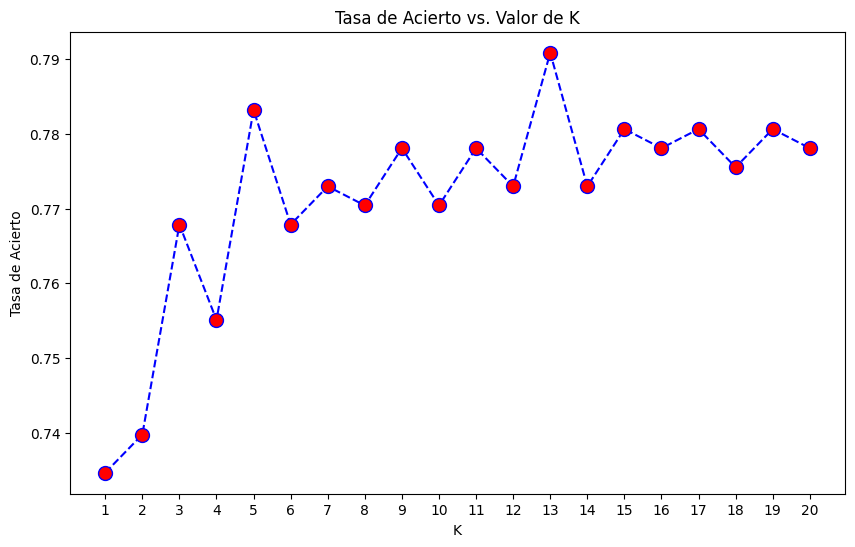
\includegraphics[width=\linewidth]{../Imagenes/Examen1/KOptimo_Estatico.png}
        \caption{Curva de acierto en función del valor de K utilizando Hold-out Validation.}
        \label{fig:Curva_Acierto_K_Holdout}
    \end{minipage}\hfill
    % \begin{minipage}{0.48\textwidth}
    %     \centering
    %     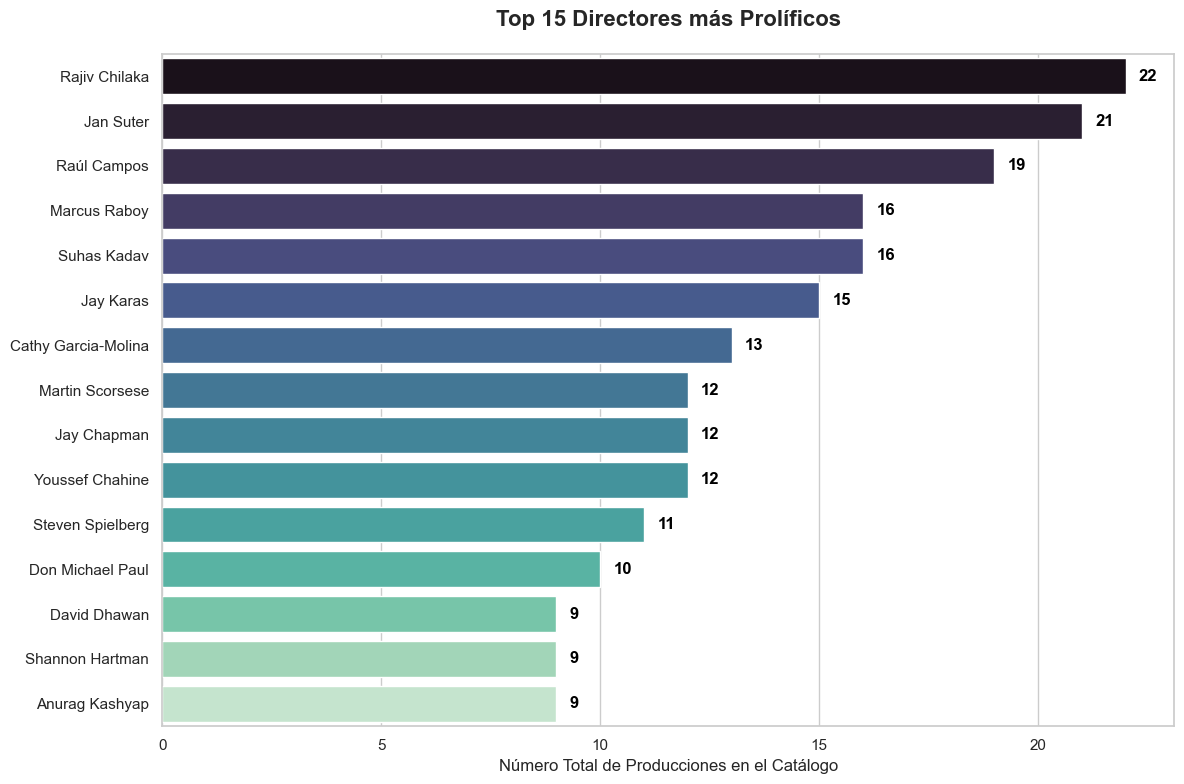
\includegraphics[width=\linewidth]{../Imagenes/Reto_2/Top15Directores.png}
    %     \caption{Top 15 Directores con más títulos.}
    %     \label{fig:top_directores}
    % \end{minipage}
\end{figure}

Con esta grafica podemos observar que el valor de K que maximiza la tasa de acierto es K=5 y K=13. Pero el valor mas cercano para probar es 5, por lo que lo empece a realizar las pruebas y observar las metricas que arroja el modelo entrenado.

\begin{figure}[H]
    \centering
    \begin{minipage}{0.48\textwidth}
        \centering
        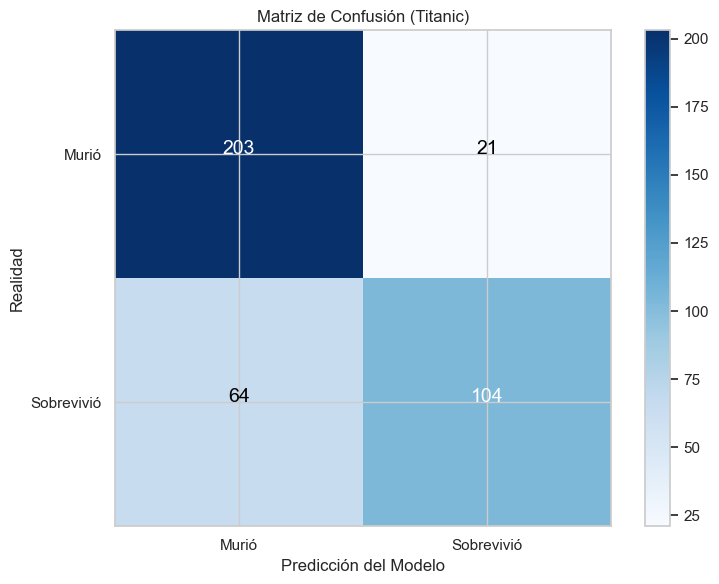
\includegraphics[width=\linewidth]{../Imagenes/Examen1/Matriz_Confusion_ModeloPrueba1.png}
        \caption{Matriz de confusión del modelo KNN con K=5 utilizando Hold-out Validation.}
        \label{fig:Matriz_Confusion_Holdout}
    \end{minipage}\hfill
    \begin{minipage}{0.48\textwidth}
        \centering
        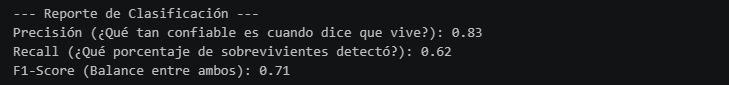
\includegraphics[width=\linewidth]{../Imagenes/Examen1/Captura de pantalla 2026-04-17 223250.png}
        \caption{Metricas de desempeño del modelo KNN con K=5 utilizando Hold-out Validation.}
        \label{fig:Metricas_Holdout}
    \end{minipage}
\end{figure}

Por lo que se puede observar las metricas que nos arrojo fue la siguiente:
\begin{itemize}
    \item Accuracy: 0.83
    \item Recall: 0.62
    \item F1-Score: 0.71
\end{itemize}

Y la distribucion de los datos se ve de la siguiente manera:
\begin{figure}[H]
    \centering
    \begin{minipage}{0.48\textwidth}
        \centering
        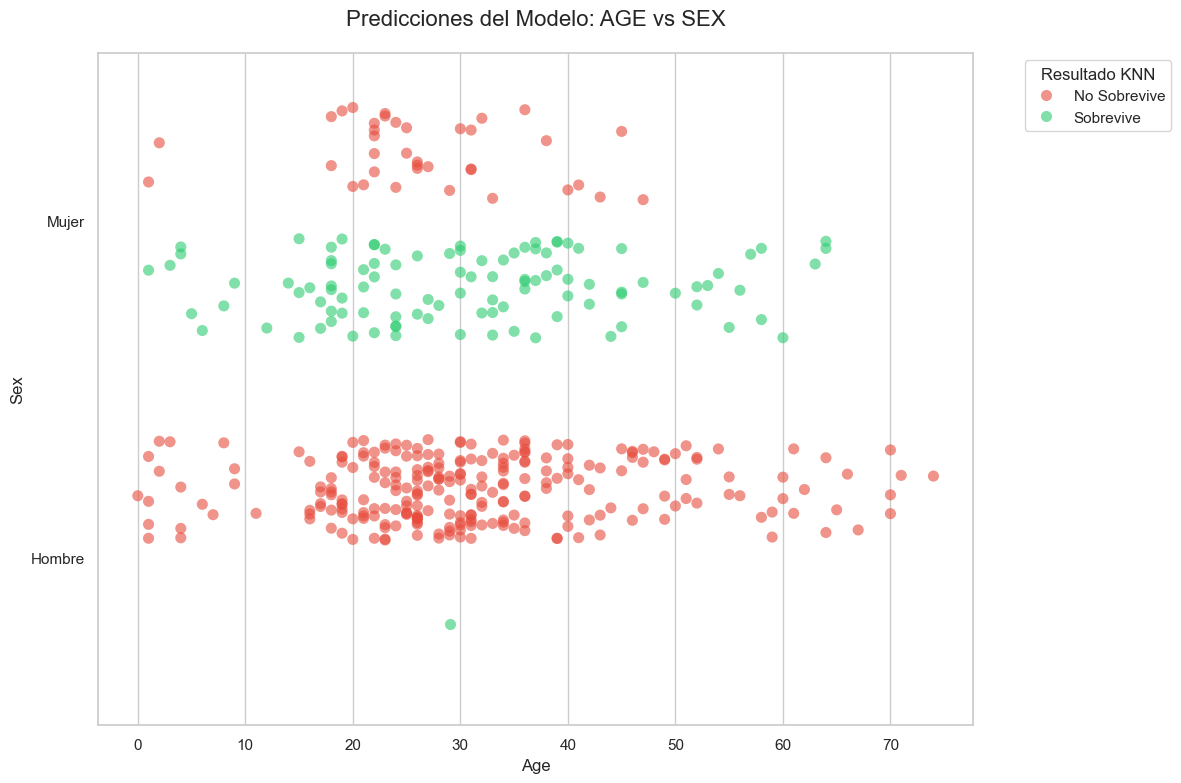
\includegraphics[width=\linewidth]{../Imagenes/Examen1/PrediccionKOptimo_prueba1_edadvsGenero.png}
        \caption{Predicciones del modelo KNN con K=5 utilizando Hold-out Validation.}
        \label{fig:Predicciones_Holdout}
    \end{minipage}\hfill
    \begin{minipage}{0.48\textwidth}
        \centering
        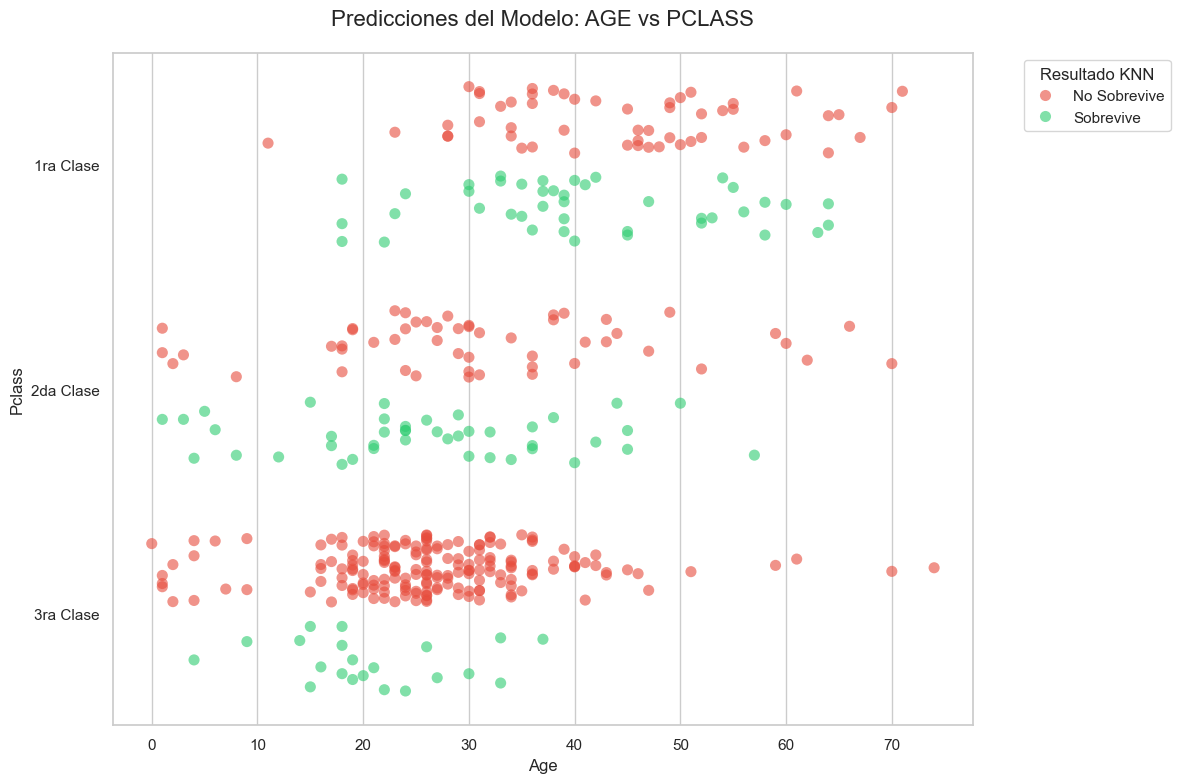
\includegraphics[width=\linewidth]{../Imagenes/Examen1/EdadvsClase_KOptimo_Pruebas1.png}
        \caption{Distribución de predicciones del modelo KNN con K=5 utilizando Hold-out Validation.}
        \label{fig:Distribucion_Predicciones_Holdout}
    \end{minipage}
\end{figure}

Como se puede observar en la \ref{fig:Predicciones_Holdout} y en la \ref{fig:Distribucion_Predicciones_Holdout} el modelo tiene una buena capacidad para identificar a los sobrevivientes, especialmente en el grupo de mujeres y niños, lo cual es consistente con los patrones visuales observados inicialmente. Sin embargo, también se puede notar que el modelo tiene dificultades para clasificar correctamente a algunos hombres adultos, lo que sugiere que podría beneficiarse de un ajuste adicional o de la incorporación de características adicionales para mejorar su capacidad de discriminación.
Por lo que ahora pasaremos a la segunda prueba, donde se implementara la validacion cruzada de K-pliegues para obtener una estimacion mas robusta del desempeño del modelo y asi poder comparar los resultados obtenidos con la tecnica de Hold-out.

\subsection{Segunda prueba.- KNN y Validación Cruzada de K-Pliegues}
En esta segunda prueba, se implementó la validación cruzada de K-pliegues para evaluar el desempeño del modelo KNN de manera más robusta. Se utilizó un valor de $K$ igual a 5 para el clasificador y se dividió el dataset en 5 pliegues. El proceso se repitió iterativamente, rotando el pliegue de prueba en cada iteración, y se registraron las métricas de desempeño para cada pliegue.
\begin{figure}[H]
    \centering
    \begin{minipage}{0.48\textwidth}
        \centering
        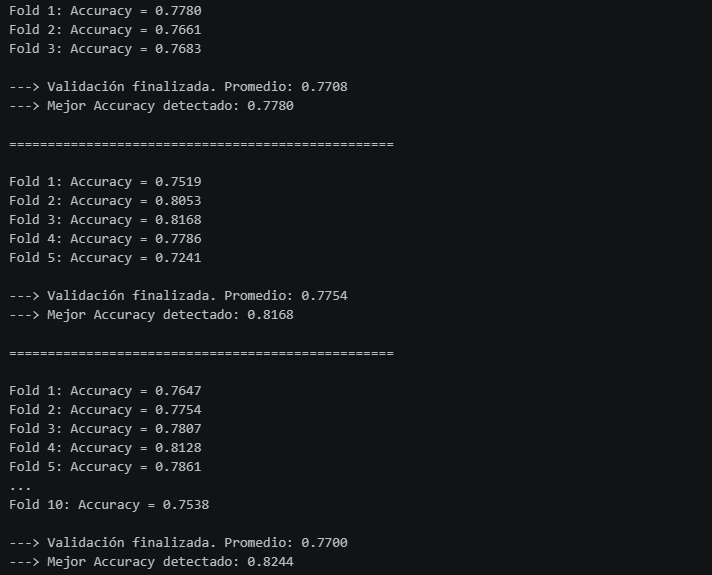
\includegraphics[width=\linewidth]{../Imagenes/Examen1/Pruebas_KFold.png}
        \caption{Curva de acierto para obtener el valor optimo de K- Fold para realizar las pruebas.}
        \label{fig:Curva_Validacion_Cruzada}
    \end{minipage}
    \end{figure}

Aqui podemos observar que el k optimo que se obtuvo fue de igual  manera 5, este valor se usara para en el codigo de la lista (\ref{lst:validacion_kfold}).
\begin{figure}[H]
    \centering
    \begin{minipage}{0.48\textwidth}
        \centering
        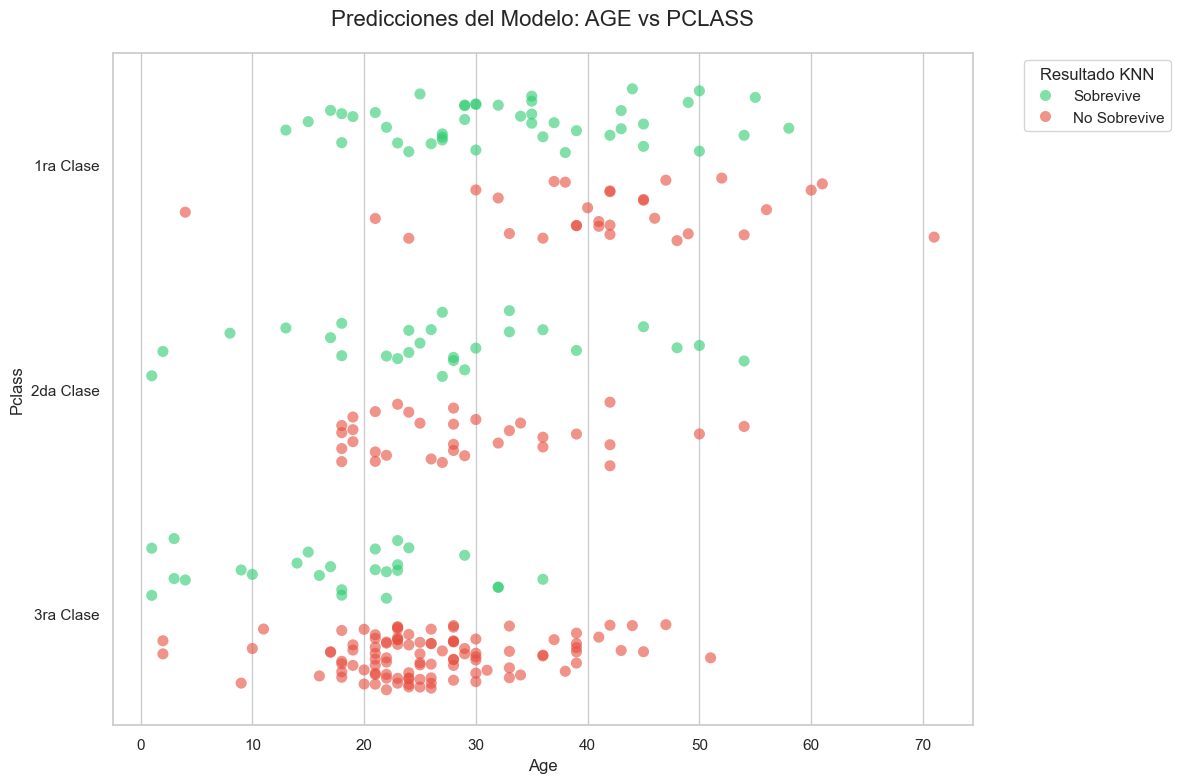
\includegraphics[width=\linewidth]{../Imagenes/Examen1/Resultado_KFoldOptimo.png}
        \caption{Prediccion del modelo KNN con K=5 utilizando Validación Cruzada de K-Pliegues. Edad vs Clase.}
        \label{fig: Predicciones_KFold_EdadGenero}
    \end{minipage}\hfill
    \begin{minipage}{0.48\textwidth}
        \centering
        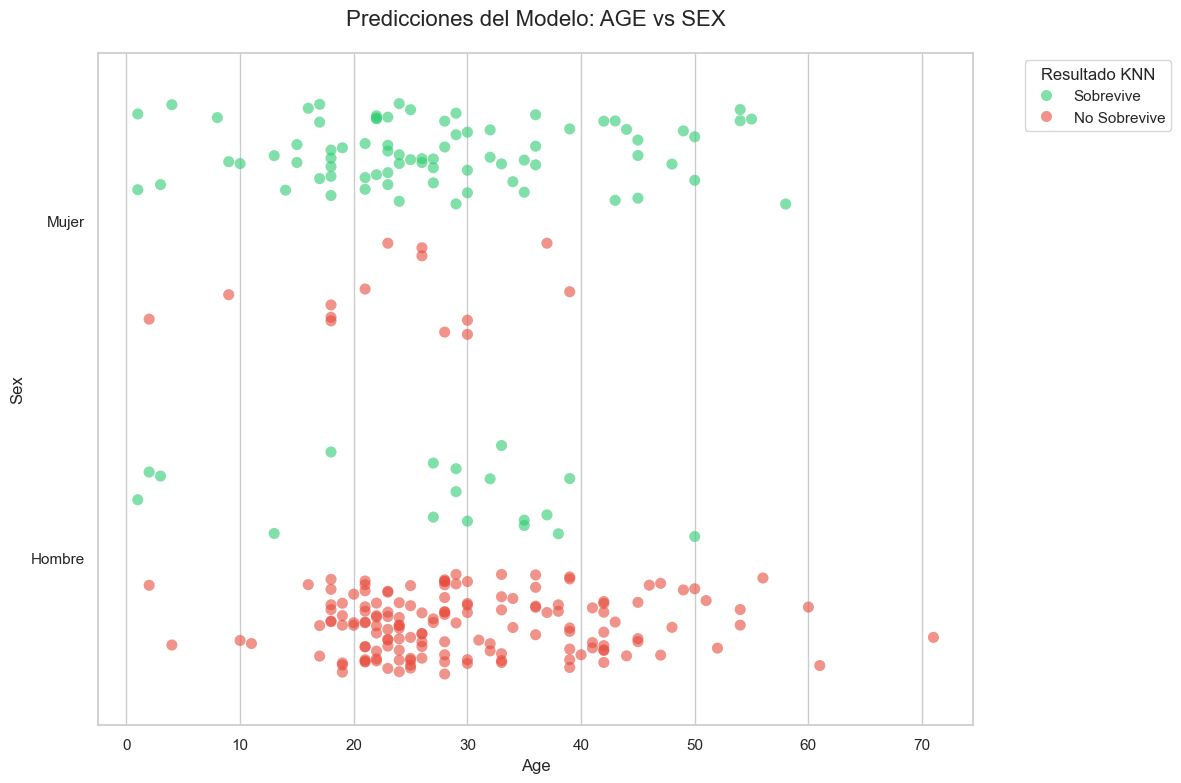
\includegraphics[width=\linewidth]{../Imagenes/Examen1/Resultado_KFoldOptimoEdadVsGenero.png}
        \caption{Predicciones del modelo KNN con K=5 utilizando Validación Cruzada de K-Pliegues.}
        \label{fig:Predicciones_KFold}
    \end{minipage}
    \end{figure}
    \begin{figure}[H]
    \centering

    \begin{minipage}{0.48\textwidth}
        \centering
        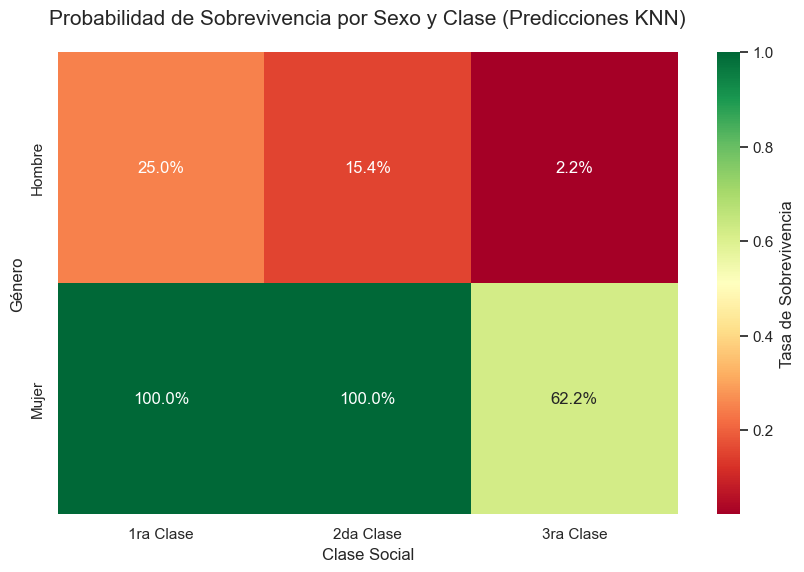
\includegraphics[width=\linewidth]{../Imagenes/Examen1/HeatMap_GeneroVsClase_KFold.png}
        \caption{Probabilidad de supervivencia del modelo KNN con K=5 utilizando Validación Cruzada de K-Pliegues. Genero vs Clase.}
        \label{fig: HeatMap_KFold_EdadClase}
    \end{minipage}\hfill
    \begin{minipage}{0.48\textwidth}
        \centering
        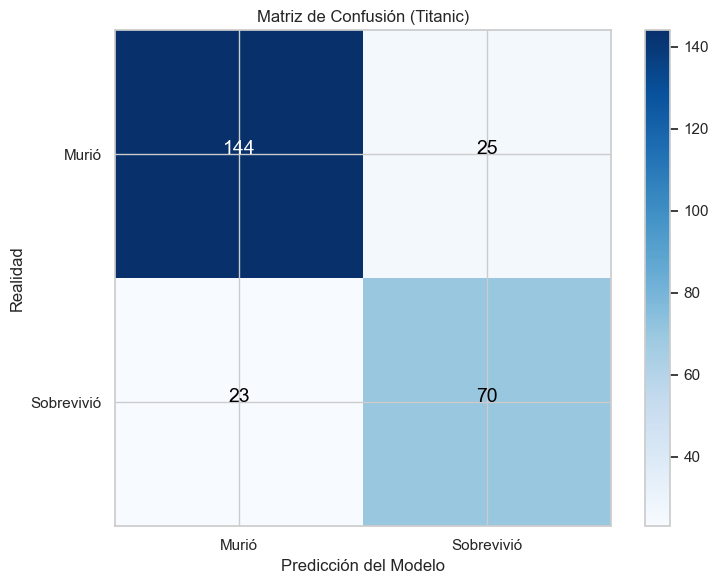
\includegraphics[width=\linewidth]{../Imagenes/Examen1/MatrizConfusion_KFoldOptimo.png}
        \caption{Matriz de Confusión del modelo KNN con K=5 utilizando Validación Cruzada de K-Pliegues.}
        \label{fig: MatrizConfusion_KFold}
    \end{minipage}
    \end{figure}

    Este mapa de calor nos da una visualización clara de cómo el modelo KNN con validación cruzada ha aprendido a asociar ciertas características con la probabilidad de supervivencia. Podemos observar que las mujeres de clase alta tienen una probabilidad significativamente mayor de sobrevivir, lo cual es consistente con los patrones históricos del desastre del Titanic. Por otro lado, los hombres adultos de clase baja presentan una probabilidad mucho menor de supervivencia, lo que también refleja la realidad histórica y valida la capacidad del modelo para capturar estas relaciones complejas entre las características de los pasajeros y su destino final.

\section{Conclusión}
En este estudio se implementó un clasificador de K-Vecinos más Cercanos (KNN) para predecir la supervivencia de los pasajeros del Titanic, utilizando tanto la técnica de Hold-out como la validación cruzada de K-pliegues para evaluar su desempeño. Los resultados obtenidos mostraron que el modelo KNN con $K=5$ logró una tasa de acierto significativa, especialmente al identificar a mujeres y niños como sobrevivientes, lo cual es coherente con los patrones históricos del desastre.
Tambien demuestra de forma muy cruda la realidad de la toma de decisiones en situaciones de emergencia, donde factores como el género y la clase social jugaron un papel crucial en la supervivencia de los pasajeros. 
Por lo tanto, este análisis no solo valida la eficacia del modelo KNN para esta tarea de clasificación, sino que también proporciona una perspectiva histórica sobre las dinámicas sociales presentes en el contexto del Titanic.

Tambien aprendi bastante en el desarrollo de este proyecto, desde la implementacion de los modelos, como tambien la forma en la que se manejan los datos de entrada, ya que vivi la experiencia de que al principio el modelo al momento de ingresar los datos de forma incorrecta las metricas de evaluacion que regresaba eran muy baja por lo que al momento de realizar la limpieza y normalizacion de los datos el modelo mejoro significativamente, esto me hizo entender la importancia de tener un buen preprocesamiento de los datos para obtener buenos resultados en el modelo.
Y tambien me di cuenta de la importancia de la validacion cruzada para obtener una estimacion mas robusta del desempeño del modelo, ya que al realizar la validacion cruzada se obtiene una mejor idea de como el modelo se comporta con diferentes particiones de los datos, lo que permite identificar si el modelo esta sobreajustado o subajustado.
En resumen, este proyecto no solo permitió aplicar técnicas de machine learning para resolver un problema de clasificación, sino que también proporcionó una comprensión más profunda de la importancia del preprocesamiento de datos y la validación cruzada en el desarrollo de modelos predictivos efectivos.

\printbibliography[title={ Bibliográficas}]
\end{document}